% Moved to section 1.4 Definitions, acronyms, abbreviations


\begin{table}[H]
    \centering
    \begin{tabular}{|l|p{0.75\textwidth}|}
        \hline % ---------------------------------------------------------------------
    	\textsc{id}                 &   1\\
    	\hline % ---------------------------------------------------------------------
    	\textsc{Name}               &   Visualize the performance data of each farmer\\
    	\hline % ---------------------------------------------------------------------
    	\textsc{Actors}             &   Policy maker\\
    	\hline % ---------------------------------------------------------------------
    	\textsc{Entry conditions}   &   Policy maker has logged in\\
    	\hline % ---------------------------------------------------------------------
    	\textsc{Event flow}         &   %\footnotesize
            	                        \begin{itemize}
                                    	    \item Policy maker presses the button “Farmer’s performance”
                                    	    \item The system displays options to let user select filters about weather type, product type
                                    		\item Policy maker selects needed filters
                                    		\item The system displays a page with list of farmer divided by performances
                                    		\item Policy maker selects interested farmer’s name
                                    		\item The system shows the detailed information about farmer’s production
                                        \end{itemize}\\
        \hline % ---------------------------------------------------------------------
        \textsc{Exit conditions}    &  The system returns to the main page of policy maker\\
    	\hline % ---------------------------------------------------------------------
    	\textsc{Output}             &  \begin{itemize}
    	    \item Policy maker has obtained the farmer's production data they were looking for
    	\end{itemize}\\
    	\hline % ---------------------------------------------------------------------
    	\textsc{Exceptions}         &  Policy maker couldn’t find the name of farmer who should exist. The system suggests the user to change the selected filter.\\
    	\hline % ---------------------------------------------------------------------
        
    \end{tabular}
    \caption{\label{tab:visualize_farmer_performance}Visualize the performance data} %TODO: add caption
\end{table}

\begin{figure}[H]
    \centering
    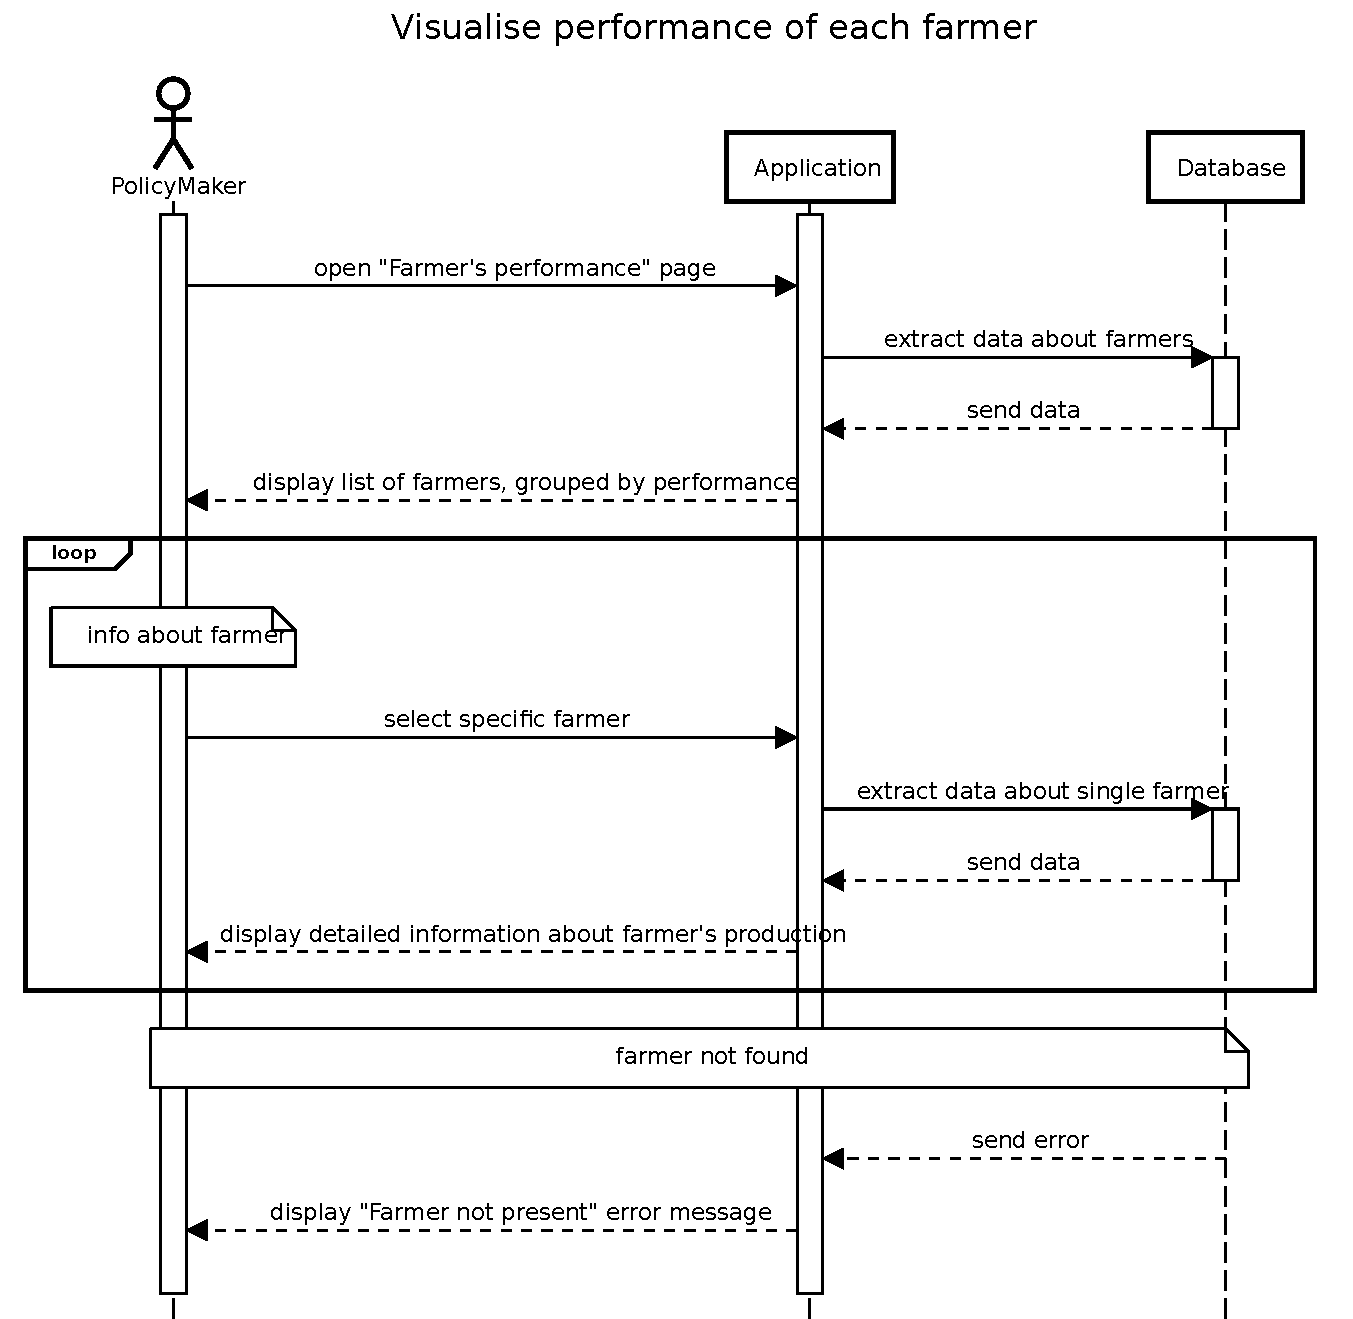
\includegraphics[scale=0.5]{Images/Sequence diagrams/PolicyMaker - visualize performance.pdf}
    \caption{Caption}
    \label{fig:my_label}
\end{figure}

\begin{table}[H]
    \centering
    \begin{tabular}{|l|p{0.75\textwidth}|}
        \hline % ---------------------------------------------------------------------
    	\textsc{id}                 &   2\\
    	\hline % ---------------------------------------------------------------------
    	\textsc{Name}               &   Manage the incentive of high performing farmer \\
    	\hline % ---------------------------------------------------------------------
    	\textsc{Actors}             &   Policy maker\\
    	\hline % ---------------------------------------------------------------------
    	\textsc{Entry conditions}   &   Policy maker has logged in\\
    	\hline % ---------------------------------------------------------------------
    	\textsc{Event flow}         &   %\footnotesize
            	                        \begin{itemize}
                                    	    \item Policy maker presses the button “Farmer’s performance”
                                    		\item The system displays a page with list of farmer divided by performance, at the place of high performer there is a column which clarifies the status of incentive 
                                       		\item Policy maker selects interested farmer’s incentive column
                                    		\item The system shows the detailed information about farmer’s incentive status
                                    		\item Policy maker clicks the incentive column
                                    		\item The system shows the possible choices
                                    		\item Policy maker selects the incentive to give
                                    		\item The system shows the popup to ask a confirmation to proceed
                                    		\item Policy maker clicks "Confirm" button
                                    		\item The system shows the updated incentive column
                                        \end{itemize}\\
        \hline % ---------------------------------------------------------------------
        \textsc{Exit conditions}    &  The system returns to the main page of policy maker\\
    	\hline % ---------------------------------------------------------------------
    	\textsc{Output}             &  \begin{itemize}
    	    \item Policy maker has managed the incentive to give
    	\end{itemize}\\
    	\hline % ---------------------------------------------------------------------
    	\textsc{Exceptions}         &  Policy maker selected an incentive data wrongly. When the 
    	system shows a popup to ask a confirmation to proceed, the policy maker can redo the operation by clicking on “Cancel” button\\
    	\hline % ---------------------------------------------------------------------
        
    \end{tabular}
    \caption{\label{tab:visualize_incentives}Manage the incentive} %TODO: add caption
\end{table}

\begin{figure}[H]
    \centering
    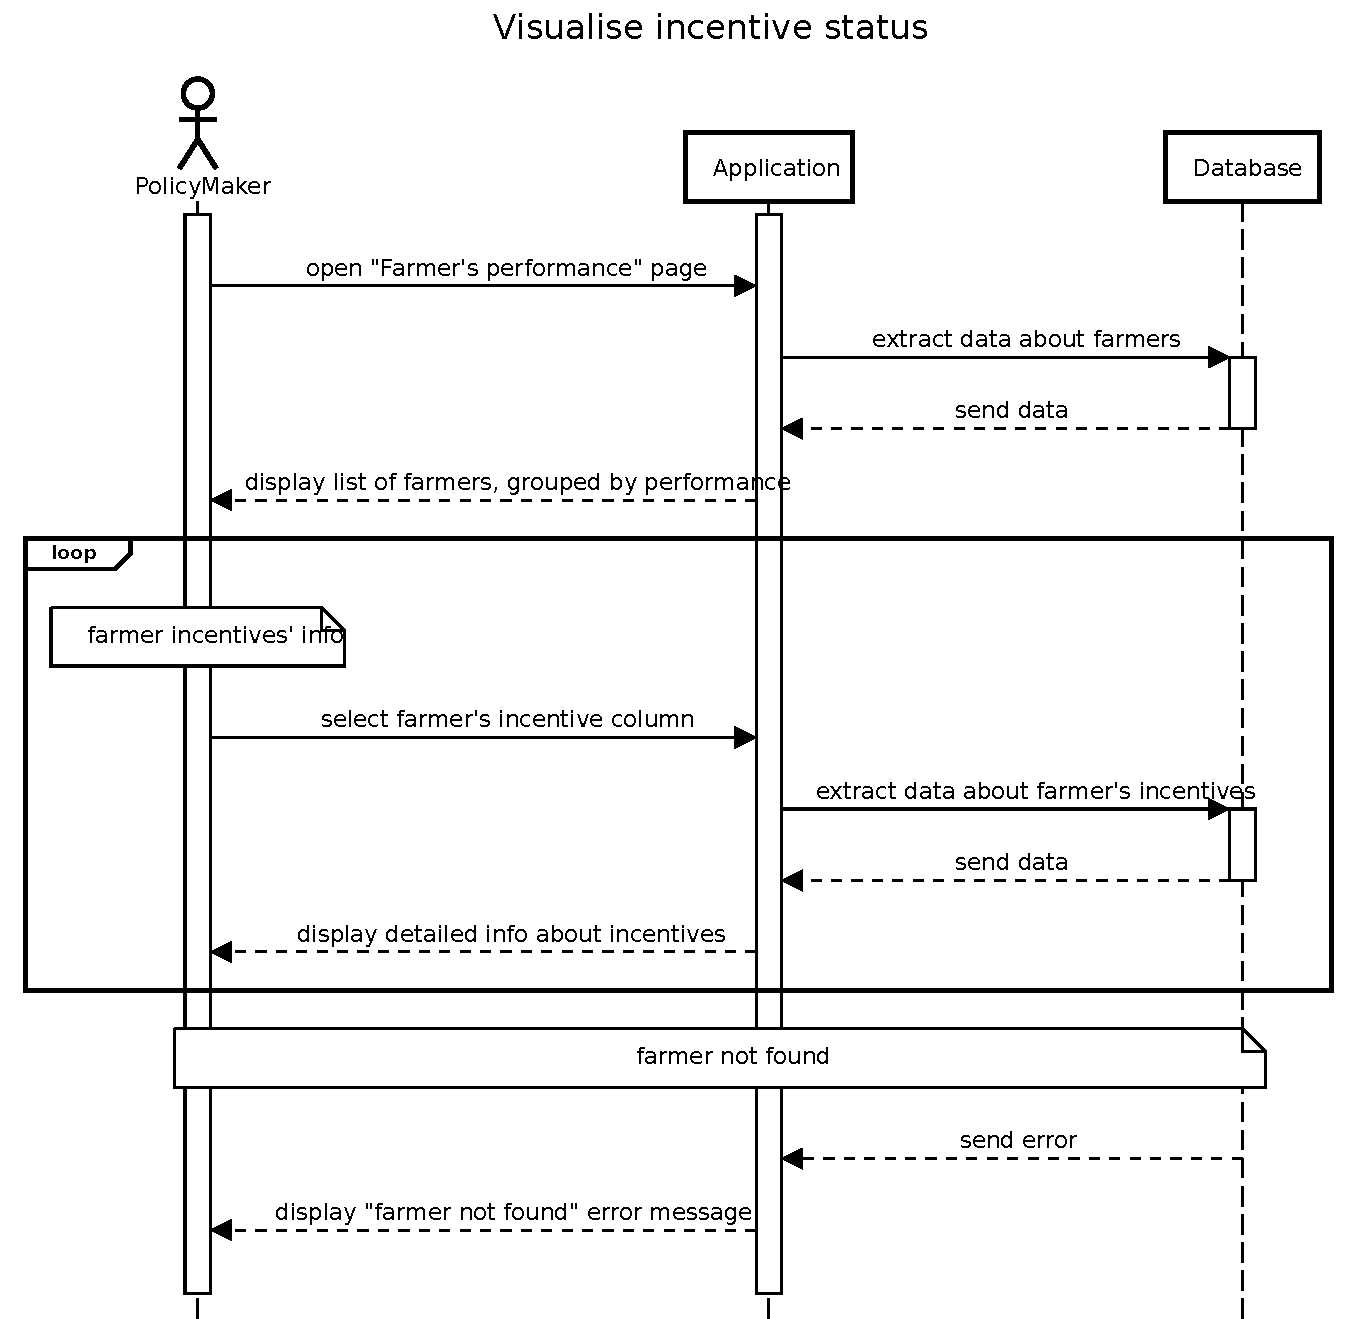
\includegraphics[scale=0.5]{Images/Sequence diagrams/PolicyMaker - visualise incentive status.pdf}
    \caption{Caption}
    \label{fig:my_label}
\end{figure}

\begin{table}[H]
    \centering
    \begin{tabular}{|l|p{0.75\textwidth}|}
        \hline % ---------------------------------------------------------------------
    	\textsc{id}                 &   3\\
    	\hline % ---------------------------------------------------------------------
    	\textsc{Name}               &   Visualize the performance difference of farmer between the current data and the past data with a history of communication done 
    	by agronomist\\
    	\hline % ---------------------------------------------------------------------
    	\textsc{Actors}             &   Policy maker\\
    	\hline % ---------------------------------------------------------------------
    	\textsc{Entry conditions}   &   Policy maker has logged in\\
    	\hline % ---------------------------------------------------------------------
    	\textsc{Event flow}         &   %\footnotesize
            	                        \begin{itemize}
                                    	    \item Policy maker presses the button “Performance transition”
                                    	    \item The system displays options to let user select filters about weather type, product type
                                    		\item Policy maker selects needed filters
                                    		\item The system displays a page with categorized farmer, also it highlights the farmers who have improved their performance significantly within a year
                                    		\item Policy maker selects interested farmer’s name
                                    		\item The system shows the detailed information about farmer’s monthly performance transition and the history of communication done by an agronomist 
                                        \end{itemize}\\
        \hline % ---------------------------------------------------------------------
        \textsc{Exit conditions}    &  The system returns to the main page of policy maker\\
    	\hline % ---------------------------------------------------------------------
    	\textsc{Output}             &  \begin{itemize}
    	    \item Policy maker has obtained the history of performance data and interaction between farmers and agronomists they were looking for
    	\end{itemize}\\
    	\hline % ---------------------------------------------------------------------
    	\textsc{Exceptions}         &  Policy maker couldn’t find the name of farmer who should exist. The system suggests the user to change the selected filter.\\
    	\hline % ---------------------------------------------------------------------
        
    \end{tabular}
    \caption{\label{tab:visualize_iprovement}Visualize the performance difference} %TODO: add caption
\end{table}

\begin{figure}[H]
    \centering
    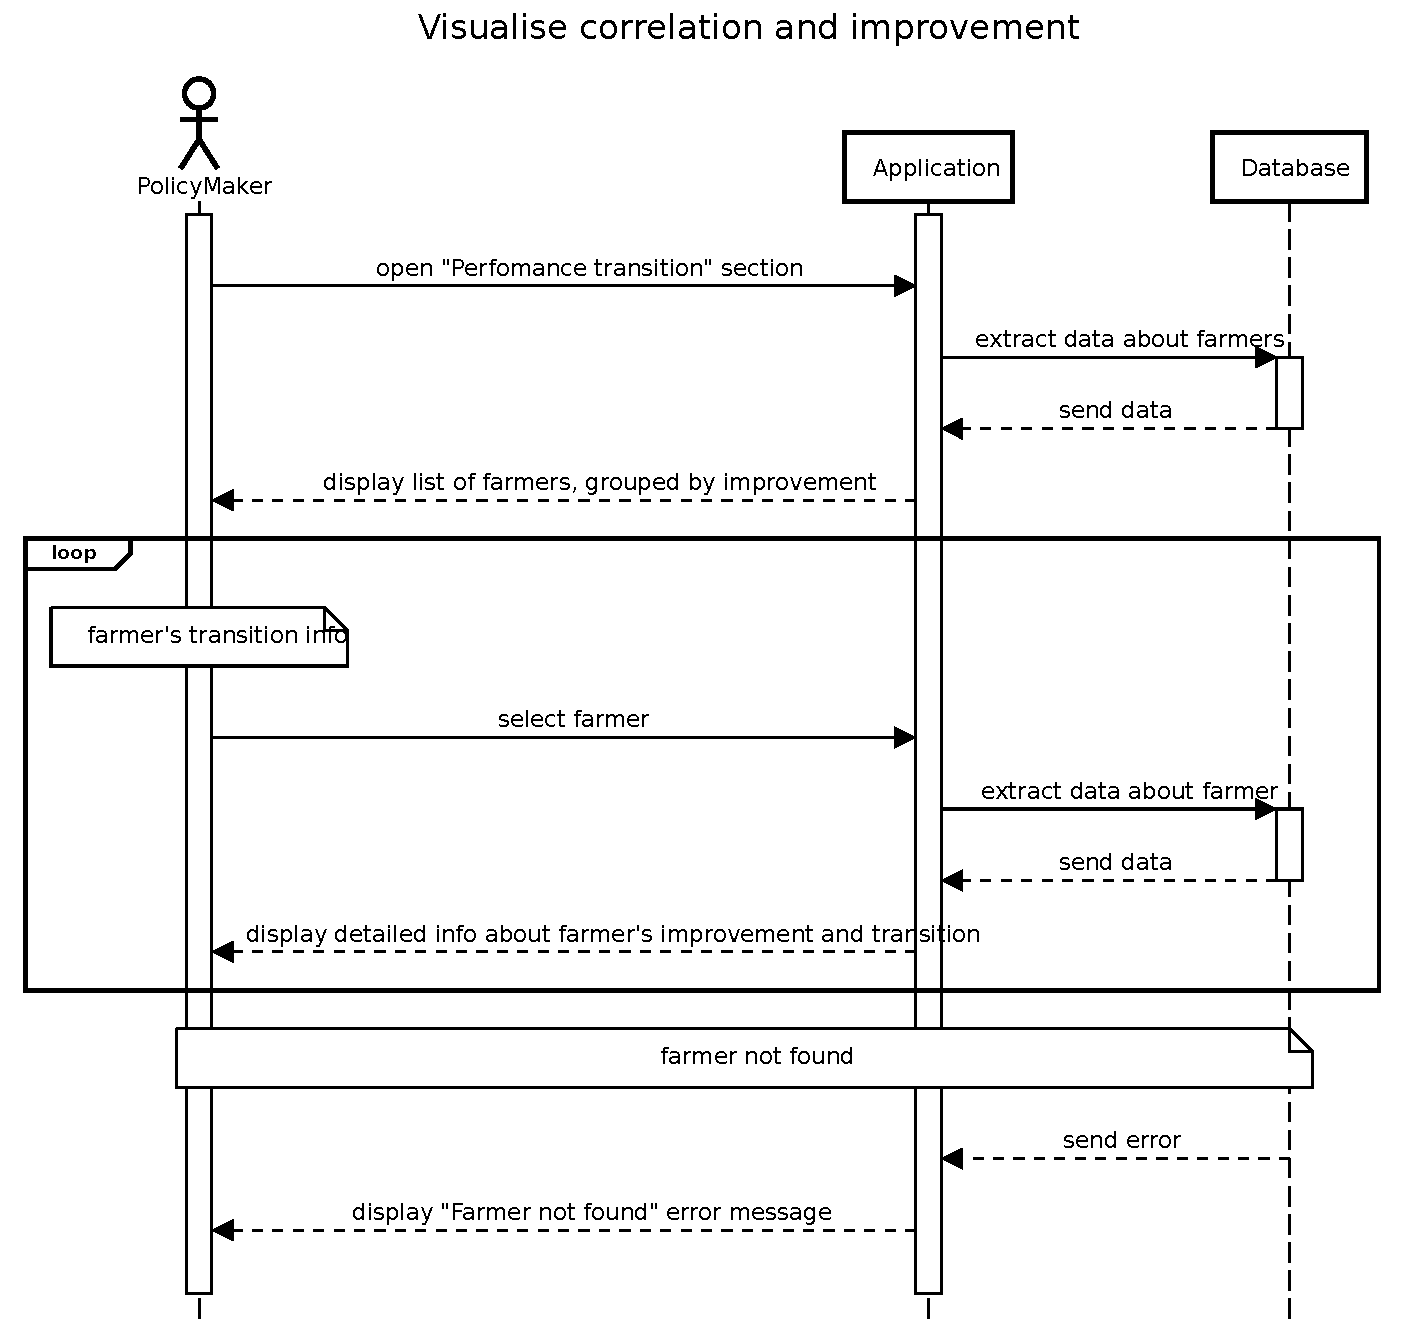
\includegraphics[scale=0.5]{Images/Sequence diagrams/PolicyMaker - visualise correlation and improvement.pdf}
    \caption{Caption}
    \label{fig:my_label}
\end{figure}

\begin{table}[H]
    \centering
    \begin{tabular}{|l|p{0.75\textwidth}|}
        \hline % ---------------------------------------------------------------------
    	\textsc{id}                 &   4\\
    	\hline % ---------------------------------------------------------------------
    	\textsc{Name}               &   Ask high performing farmers to write good practices\\
    	\hline % ---------------------------------------------------------------------
    	\textsc{Actors}             &   Policy maker\\
    	\hline % ---------------------------------------------------------------------
    	\textsc{Entry conditions}   &   Policy maker has logged in\\
    	\hline % ---------------------------------------------------------------------
    	\textsc{Event flow}         &   %\footnotesize
            	                        \begin{itemize}
                                    	    \item Policy maker presses the button “Farmer’s performance”
                                    		\item The system displays a page with list of farmer divided by performances
                                    		\item Policy maker selects interested high performing farmer’s name
                                    		\item The system shows the detailed information about farmer’s production and "request writing" button
                                    		\item Policy maker clicks "request writing" button
                                    		\item The system shows the popup to ask a confirmation to proceed
                                    		\item Policy maker clicks "Confirm" button
                                    		\item The system sends the request to the selected farmer and shows the message "request had been sent" 
                                        \end{itemize}\\
        \hline % ---------------------------------------------------------------------
        \textsc{Exit conditions}    &  The system returns to the Farmer’s performance page\\
    	\hline % ---------------------------------------------------------------------
    	\textsc{Output}             &  \begin{itemize}
    	    \item Policy maker has requested the high performing farmer to write their good practice
    	\end{itemize}\\
    	\hline % ---------------------------------------------------------------------
    	\textsc{Exceptions}         &  Policy maker selected a farmer wrongly. When the 
    	system shows a popup to ask a confirmation to proceed, the policy maker can redo the operation by clicking on “Cancel” button\\
    	\hline % ---------------------------------------------------------------------
        
    \end{tabular}
    \caption{\label{tab:visualize_iprovement}Ask a request for writing good practices} %TODO: add caption
\end{table}